\chapter{مدل‌سازی محیط یادگیری سه‌ جسمی}
مسیرهای فضایی سنتی تحت تأثیر گرانش یک جسم مرکزی (خورشید، زمین یا سیاره‌ای دیگر) شکل می‌گیرند و توسط اجسام سوم تحت تأثیر قرار می‌گیرند. تحلیل‌های مخروطی پیوسته نشان می‌دهند که چگونه می‌توان طراحی را از یک جسم مرکزی به جسم دیگر منتقل کرد، هنگامی که فضاپیما از حوزه تأثیر یک جسم عبور می‌کند. در برخی موارد، مأموریت فضاپیما آن را در ناحیه‌ای از فضا قرار می‌دهد که به‌طور همزمان تحت تأثیر دو جسم بزرگ است. این مسیرها نمی‌توانند از تحلیل دو جسم با اختلالات جسم سوم استفاده کنند، بلکه باید تأثیرات هر دو جسم به‌طور همزمان در نظر گرفته شوند. برای درک این مسئله، ابتدا به مطالعه مسئله عمومی سه‌جسمی خواهیم پرداخت و چگونگی اعمال آن به سیستم‌های واقعی را بررسی خواهیم کرد. سپس، برخی از مسیرها و تحلیل‌های جالبی که توسط فضاپیماهای مدرن استفاده می‌شوند، ارائه خواهیم داد.

در فصل اول معادلات عمومی حرکت اجسام متعدد را معرفی کردیم. علی‌رغم وجود ده ثابت حرکت، هیچ‌کس نتوانسته است مسئله عمومی سه‌جسمی را به‌صورت تحلیلی بسته حل کند—ممکن است که این کار غیرممکن باشد. بنابراین، تحقیقات بر روی ساده‌سازی مسئله عمومی متمرکز شده است. ساندمن در سال 1912 یک راه‌حل سری توانی یافت. زمانی که این راه‌حل با شرایط اولیه ترکیب شود، ارزیابی‌های عددی از مسیرها را در یک بازه زمانی محدود ارائه می‌دهد. برای مطالعه کامل مسئله، به کتاب Szebehely (1967) مراجعه کنید. یکی از راه‌حل‌های تحلیلی خاص—مسئله سه‌جسمی محدود—از زمان اویلر و لاگرانژ شناخته شده است. اخیراً، از تکنیک‌های عددی برای تولید راه‌حل‌ها استفاده شده است.

دانشمندان برای صدها سال مسئله سه‌جسمی را مطالعه کرده‌اند، اگرچه بیشتر تحقیقات از دهه 1960، با استفاده از فناوری محاسباتی مدرن، انجام شده است. تحلیل‌های آنها انواع مختلفی از مدارهای سه‌جسمی را کشف کرده است که بسیاری از آنها برای فضاپیماها بسیار مفید هستند. در این بخش، چندین گزینه مدار سه‌جسمی را بررسی خواهیم کرد.



\pgfmathsetmacro{\r}{0.8}	
\pgfmathsetmacro{\Phi}{-160}
\pgfmathsetmacro{\Theta}{-90}

\section{مسئله‌ی سه‌جسمیِ محدودِ دایره‌ای (\lr{CRTBP})}\label{sec:crtbp}

دو جرمِ اصلی (زمین
با جرم~$m_{1}$ و ماه با جرم~$m_{2}$) روی مدارهایی دایره‌ای و هم‌صفحه پیرامونِ مرکزِ جرمِ مشترک حرکت می‌کنند. جرمِ سوم (فضاپیما با جرمِ ناچیز $m_{3}$) چنان کوچک فرض می‌شود که تأثیرِ گرانشیِ آن بر حرکتِ دو جسمِ اصلی قابل صرفِ نظر است؛ بدین ترتیب، مسئله‌ی سه‌جسمیِ محدودِ دایره‌ای شکل می‌گیرد.



\begin{table}[H]
	\centering
	\caption{مقادیر عددی برای مسئله سه‌جسمی محدود (سامانه زمین–ماه)}
	\begin{tabular}{|c|c|c|}
		\hline
		پارامتر & توصیف & مقدار عددی \\
		\hline
		$m_1$ & جرم زمین & $5.972 \times 10^{24}\,\mathrm{kg}$ \\
		$m_2$ & جرم ماه & $7.348 \times 10^{22}\,\mathrm{kg}$ \\
		$\mu$ & نسبت جرمی & $0.0121505856$ \\
		$\omega$ & سرعت زاویه‌ای سامانه & $2.6617 \times 10^{-6}\,\mathrm{rad/s}$ \\
		\hline
	\end{tabular}
	\label{tab:params}
\end{table}



دستگاهِ مختصاتِ چرخانی هم‌دوران با دو جرم اصلی انتخاب می‌شود؛ مبدأ در مرکزِ جرمِ سامانه است، محور~$x$ خطِ واصلِ دو جرم و محور~$y$ بر آن عمود (در صفحه‌ی مدارها) است. واحدِ طول برابر فاصله‌ی ثابتِ میان دو جرم و واحدِ زمان چنان تعریف می‌شود که دوره‌ی مداریِ سامانه $2\pi$ (و در نتیجه $\omega=1$) گردد. همچنین جرم‌ها به‌گونه‌ای مقیاس می‌شود که مجموع دو جرم برابر با یک شود:
\begin{equation}
	 m_{1}+m_{2}=1.
\end{equation}
با نسبتِ جرمی
\begin{equation}
	\mu\equiv\frac{m_{2}}{m_{1}+m_{2}},
\end{equation}
داریم $m_{1}=1-\mu$ و $m_{2}=\mu$ و مکانِ دو جرم در دستگاهِ بی‌بُعد به صورت
\begin{equation}
	\mathbf r_{\text{Earth}}=(-\mu,0),\qquad \mathbf r_{\text{Moon}}=(1-\mu,0).
\end{equation}


\begin{figure}[H]
\centering
\begin{tikzpicture}
	% Coordinates
	\coordinate (earth) at (1,2);
	\coordinate (moon) at (8,1);
	\coordinate (earth-point1) at ({\r*cos(\Theta)+1},{\r*sin(\Theta)+2});
	\coordinate (A) at (-.5,.5);
	\coordinate (B) at (8.5,-0.5);
	
	% Earth
	\draw[thick, fill=black!30, draw=black!30
	] (earth) circle (\r);
	\node[inner sep=0pt] (Earth_c) at (earth) {
\includegraphics[width=1.8cm]{../Figure/TBP/Earth.png}};
	% Text
	\node[below, shift={(0,-0.8)}] at (earth) {$m_1$};
	\node (a) at (A) {زمین};
	
	% Moon
	\node[circle, inner sep=5.5pt, fill=black!30] (MOON) at (moon) {};
	\node[inner sep=0pt] (moon_c) at (moon) {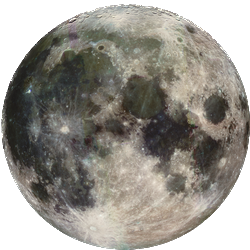
\includegraphics[width=.5cm]{../Figure/TBP/Moon.png}};
	% Text 
	\node[below, shift={(0,-0.4)}] at (MOON) {$m_2$};
	\node (b) at (B) {ماه};
	
	% Lines
	\draw[-stealth] (a) to[bend left=30] ({\r*cos(\Phi)+1},{\r*sin(\Phi)+2});
	\draw[-stealth] (b) to[bend left=-30] (MOON);
	\draw[dashed, black] (earth) -- (MOON.center);
	
	% center of mass 0.25 from earth
	\coordinate (center) at ($(earth)!0.3!(MOON)$);
	% small circle
	\draw[fill=black] (center) circle (1.5pt) node[below, shift={(0,-0.1)}] {جرم مرکز };
	
	% Calculate direction from Earth to Moon
	\pgfmathsetmacro{\xDiff}{8 - 1} % X difference between Moon and Earth
	\pgfmathsetmacro{\yDiff}{1 - 2} % Y difference between Moon and Earth
	\pgfmathsetmacro{\angle}{atan2(\yDiff,\xDiff)} % Angle of the line
	
	% Add axes at center of mass
	\draw[->, thick] (center) -- ++(\angle:2) node[above, shift={(0,0.2)}] {محور $x$};
	\draw[->, thick] (center) -- ++(\angle+90:2) node[above] {محور $y$};
	
	% add satellite with shift
	\coordinate (satellite) at ($(center)!0.5!(MOON)+(0,2)$);
	\node (satellite) at (satellite) {\faSatellite};
	
	% connect earth to satellite r1
	\draw[-stealth] (earth) -- (satellite) node[pos=0.3, above] {$\vb{r}_1$};   
	% connect moon to satellite r2
	\draw[-stealth] (MOON) -- (satellite) node[pos=0.5, above] {$\vb{r}_2$};
	% connect center of mass to satellite r
	\draw[-stealth] (center) -- (satellite) node[pos=0.5, above] {$\vb{r}$};
	% add line to show satellite is in between
	\node (c) at ($(satellite)+(1.5,0.5)$) {فضاپیما};
	\draw[-stealth] (c) to[bend left=30] (satellite);
	
\end{tikzpicture}
\caption{هندسه‌ی مسئله‌ی سه‌جسمیِ محدود در چارچوبِ چرخان}
\end{figure}



\subsection{لاگرانژ و معادلات حرکت}
با در نظر گرفتن
$G=1$
در حالت بی‌بُعد،
تابعِ لاگرانژِ جرمِ سوم در دستگاهِ چرخان برابر است با\cite{vallado2001fundamentals}
\begin{equation}\label{eq:L_crtbp}
	L=\tfrac12\bigl(\dot x^{2}+\dot y^{2}+\dot z^{2}\bigr)
	+(1-\mu)\,\frac{1}{r_{1}}+\mu\,\frac{1}{r_{2}}
	+\tfrac12\bigl(x^{2}+y^{2}\bigr),
\end{equation}
که در آن
\begin{equation}
	r_{1}=\sqrt{(x+\mu)^{2}+y^{2}+z^{2}},\qquad
	r_{2}=\sqrt{\bigl(x-1+\mu\bigr)^{2}+y^{2}+z^{2}}.
\end{equation}

با به‌کارگیری رابطه‌ی اویلر–لاگرانژ
\begin{equation*}
	\frac{\mathrm d}{\mathrm dt}\frac{\partial L}{\partial \dot q_{i}}-
	\frac{\partial L}{\partial q_{i}}=0,\qquad q_{i}\in\{x,y,z\},
\end{equation*}
معادلاتِ بی‌بُعدِ حرکتِ جرمِ سوم به دست می‌آید:
\begin{align}
	\ddot x-2\dot y &=
	x-\frac{1-\mu}{r_{1}^{3}}(x+\mu)-\frac{\mu}{r_{2}^{3}}\bigl(x-1+\mu\bigr),\\[2pt]
	\ddot y+2\dot x &=
	y-\frac{1-\mu}{r_{1}^{3}}\,y-\frac{\mu}{r_{2}^{3}}\,y,\\[2pt]
	\ddot z &= -\frac{1-\mu}{r_{1}^{3}}\,z-\frac{\mu}{r_{2}^{3}}\,z.
\end{align}
یا به نگاشتِ برداری به‌صورت زیر است.
\begin{equation}
	\ddot{\mathbf r}+2\,\boldsymbol\omega\times\dot{\mathbf r}=\nabla\Omega(\mathbf r),\qquad
	\Omega(x,y,z)=\tfrac12\bigl(x^{2}+y^{2}\bigr)+\frac{1-\mu}{r_{1}}+\frac{\mu}{r_{2}}.
\end{equation}
که در آن $\Omega$ پتانسیلِ مؤثر است و در بخش \ref{sec:lag-points} برای یافتنِ نقاطِ تعادل از شرطِ $\nabla\Omega=0$ استفاده می‌شود.
%ترم‌های کورولیس~$\pm2\,\dot{\vphantom y}$ پیامد استفاده از چارچوبِ چرخان است.
